



<!DOCTYPE html>
<html lang="en" class=" is-copy-enabled is-u2f-enabled">
  <head prefix="og: http://ogp.me/ns# fb: http://ogp.me/ns/fb# object: http://ogp.me/ns/object# article: http://ogp.me/ns/article# profile: http://ogp.me/ns/profile#">
    <meta charset='utf-8'>

    <link crossorigin="anonymous" href="https://assets-cdn.github.com/assets/github-7d986e67a833be502d53614d9272115bc1f05240176c17f31d63739845349cf3.css" integrity="sha256-fZhuZ6gzvlAtU2FNknIRW8HwUkAXbBfzHWNzmEU0nPM=" media="all" rel="stylesheet" />
    <link crossorigin="anonymous" href="https://assets-cdn.github.com/assets/github2-26778d4c4a1040cca1cfe59166f2c1d1d809f6963a625f45718b7f00fe364e9d.css" integrity="sha256-JneNTEoQQMyhz+WRZvLB0dgJ9pY6Yl9FcYt/AP42Tp0=" media="all" rel="stylesheet" />
    
    
    

    <link as="script" href="https://assets-cdn.github.com/assets/frameworks-bebe77cf3c6ad6033e7df85a57952b158d1d0fadbe3590af19a960b00413bbec.js" rel="preload" />
    <link as="script" href="https://assets-cdn.github.com/assets/github-905189691a6028f88cd80210851a8dde5035886fe94a7dcd64c853a342d165fc.js" rel="preload" />

    <meta http-equiv="X-UA-Compatible" content="IE=edge">
    <meta http-equiv="Content-Language" content="en">
    <meta name="viewport" content="width=1020">
    
    
    <title>ximeraMajoringInMathematics/payingOffDebt.tex at master · bartsnapp/ximeraMajoringInMathematics · GitHub</title>
    <link rel="search" type="application/opensearchdescription+xml" href="/opensearch.xml" title="GitHub">
    <link rel="fluid-icon" href="https://github.com/fluidicon.png" title="GitHub">
    <link rel="apple-touch-icon" href="/apple-touch-icon.png">
    <link rel="apple-touch-icon" sizes="57x57" href="/apple-touch-icon-57x57.png">
    <link rel="apple-touch-icon" sizes="60x60" href="/apple-touch-icon-60x60.png">
    <link rel="apple-touch-icon" sizes="72x72" href="/apple-touch-icon-72x72.png">
    <link rel="apple-touch-icon" sizes="76x76" href="/apple-touch-icon-76x76.png">
    <link rel="apple-touch-icon" sizes="114x114" href="/apple-touch-icon-114x114.png">
    <link rel="apple-touch-icon" sizes="120x120" href="/apple-touch-icon-120x120.png">
    <link rel="apple-touch-icon" sizes="144x144" href="/apple-touch-icon-144x144.png">
    <link rel="apple-touch-icon" sizes="152x152" href="/apple-touch-icon-152x152.png">
    <link rel="apple-touch-icon" sizes="180x180" href="/apple-touch-icon-180x180.png">
    <meta property="fb:app_id" content="1401488693436528">

      <meta content="https://avatars3.githubusercontent.com/u/1376703?v=3&amp;s=400" name="twitter:image:src" /><meta content="@github" name="twitter:site" /><meta content="summary" name="twitter:card" /><meta content="bartsnapp/ximeraMajoringInMathematics" name="twitter:title" /><meta content="Contribute to ximeraMajoringInMathematics development by creating an account on GitHub." name="twitter:description" />
      <meta content="https://avatars3.githubusercontent.com/u/1376703?v=3&amp;s=400" property="og:image" /><meta content="GitHub" property="og:site_name" /><meta content="object" property="og:type" /><meta content="bartsnapp/ximeraMajoringInMathematics" property="og:title" /><meta content="https://github.com/bartsnapp/ximeraMajoringInMathematics" property="og:url" /><meta content="Contribute to ximeraMajoringInMathematics development by creating an account on GitHub." property="og:description" />
      <meta name="browser-stats-url" content="https://api.github.com/_private/browser/stats">
    <meta name="browser-errors-url" content="https://api.github.com/_private/browser/errors">
    <link rel="assets" href="https://assets-cdn.github.com/">
    
    <meta name="pjax-timeout" content="1000">
    

    <meta name="msapplication-TileImage" content="/windows-tile.png">
    <meta name="msapplication-TileColor" content="#ffffff">
    <meta name="selected-link" value="repo_source" data-pjax-transient>

    <meta name="google-site-verification" content="KT5gs8h0wvaagLKAVWq8bbeNwnZZK1r1XQysX3xurLU">
<meta name="google-site-verification" content="ZzhVyEFwb7w3e0-uOTltm8Jsck2F5StVihD0exw2fsA">
    <meta name="google-analytics" content="UA-3769691-2">

<meta content="collector.githubapp.com" name="octolytics-host" /><meta content="github" name="octolytics-app-id" /><meta content="8CFE5E69:4C10:A29302F:56CCA5E0" name="octolytics-dimension-request_id" />
<meta content="/&lt;user-name&gt;/&lt;repo-name&gt;/blob/show" data-pjax-transient="true" name="analytics-location" />



  <meta class="js-ga-set" name="dimension1" content="Logged Out">



        <meta name="hostname" content="github.com">
    <meta name="user-login" content="">

        <meta name="expected-hostname" content="github.com">
      <meta name="js-proxy-site-detection-payload" content="MDUzZGQwMDEwMmU1NDcwZDZjZjMxMzQyOWIxNzYyZTI2MDVhMTIyMjgzNWI0MmE1YmYzZWM5ODRiYTI0ZDA2ZHx7InJlbW90ZV9hZGRyZXNzIjoiMTQwLjI1NC45NC4xMDUiLCJyZXF1ZXN0X2lkIjoiOENGRTVFNjk6NEMxMDpBMjkzMDJGOjU2Q0NBNUUwIn0=">

      <link rel="mask-icon" href="https://assets-cdn.github.com/pinned-octocat.svg" color="#4078c0">
      <link rel="icon" type="image/x-icon" href="https://assets-cdn.github.com/favicon.ico">

    <meta content="45c5583527f226e6f960031f5cb634d717be2cb7" name="form-nonce" />

    <meta http-equiv="x-pjax-version" content="59f6ac20db143272097f1f3bdfdb942d">
    

      
  <meta name="description" content="Contribute to ximeraMajoringInMathematics development by creating an account on GitHub.">
  <meta name="go-import" content="github.com/bartsnapp/ximeraMajoringInMathematics git https://github.com/bartsnapp/ximeraMajoringInMathematics.git">

  <meta content="1376703" name="octolytics-dimension-user_id" /><meta content="bartsnapp" name="octolytics-dimension-user_login" /><meta content="19545538" name="octolytics-dimension-repository_id" /><meta content="bartsnapp/ximeraMajoringInMathematics" name="octolytics-dimension-repository_nwo" /><meta content="true" name="octolytics-dimension-repository_public" /><meta content="false" name="octolytics-dimension-repository_is_fork" /><meta content="19545538" name="octolytics-dimension-repository_network_root_id" /><meta content="bartsnapp/ximeraMajoringInMathematics" name="octolytics-dimension-repository_network_root_nwo" />
  <link href="https://github.com/bartsnapp/ximeraMajoringInMathematics/commits/master.atom" rel="alternate" title="Recent Commits to ximeraMajoringInMathematics:master" type="application/atom+xml">


      <link rel="canonical" href="https://github.com/bartsnapp/ximeraMajoringInMathematics/blob/master/payingOffDebt/payingOffDebt.tex" data-pjax-transient>
  </head>


  <body class="logged_out   env-production windows vis-public page-blob">
    <a href="#start-of-content" tabindex="1" class="accessibility-aid js-skip-to-content">Skip to content</a>

    
    
    



      
      <div class="header header-logged-out" role="banner">
  <div class="container clearfix">

    <a class="header-logo-wordmark" href="https://github.com/" data-ga-click="(Logged out) Header, go to homepage, icon:logo-wordmark">
      <svg aria-hidden="true" class="octicon octicon-logo-github" height="28" role="img" version="1.1" viewBox="0 0 45 16" width="78"><path d="M8.64 5.19H4.88c-0.11 0-0.19 0.08-0.19 0.17v1.84c0 0.09 0.08 0.17 0.19 0.17h1.47v2.3s-0.33 0.11-1.25 0.11c-1.08 0-2.58-0.39-2.58-3.7s1.58-3.73 3.05-3.73c1.27 0 1.81 0.22 2.17 0.33 0.11 0.03 0.2-0.08 0.2-0.17l0.42-1.78c0-0.05-0.02-0.09-0.06-0.14-0.14-0.09-1.02-0.58-3.2-0.58C2.58 0 0 1.06 0 6.2s2.95 5.92 5.44 5.92c2.06 0 3.31-0.89 3.31-0.89 0.05-0.02 0.06-0.09 0.06-0.13V5.36c0-0.09-0.08-0.17-0.19-0.17h0.02zM27.7 0.44h-2.13c-0.09 0-0.17 0.08-0.17 0.17v4.09h-3.31V0.61c0-0.09-0.08-0.17-0.17-0.17h-2.13c-0.09 0-0.17 0.08-0.17 0.17v11.11c0 0.09 0.09 0.17 0.17 0.17h2.13c0.09 0 0.17-0.08 0.17-0.17V6.97h3.31l-0.02 4.75c0 0.09 0.08 0.17 0.17 0.17h2.13c0.09 0 0.17-0.08 0.17-0.17V0.61c0-0.09-0.08-0.17-0.17-0.17h0.02zM11.19 0.69c-0.77 0-1.38 0.61-1.38 1.38s0.61 1.38 1.38 1.38c0.75 0 1.36-0.61 1.36-1.38s-0.61-1.38-1.36-1.38z m1.22 3.55c0-0.09-0.08-0.17-0.17-0.17H10.11c-0.09 0-0.17 0.09-0.17 0.2 0 0 0 6.17 0 7.34 0 0.2 0.13 0.27 0.3 0.27 0 0 0.91 0 1.92 0 0.2 0 0.25-0.09 0.25-0.27 0-0.39 0-7.36 0-7.36v-0.02z m23.52-0.16h-2.09c-0.11 0-0.17 0.08-0.17 0.19v5.44s-0.55 0.39-1.3 0.39-0.97-0.34-0.97-1.09c0-0.73 0-4.75 0-4.75 0-0.09-0.08-0.17-0.17-0.17h-2.14c-0.09 0-0.17 0.08-0.17 0.17 0 0 0 2.91 0 5.11s1.23 2.75 2.92 2.75c1.39 0 2.52-0.77 2.52-0.77s0.05 0.39 0.08 0.45c0.02 0.05 0.09 0.09 0.16 0.09h1.34c0.11 0 0.17-0.08 0.17-0.17l0.02-7.47c0-0.09-0.08-0.17-0.19-0.17z m5.77-0.25c-1.2 0-2.02 0.53-2.02 0.53V0.59c0-0.09-0.08-0.17-0.17-0.17h-2.13c-0.09 0-0.17 0.08-0.17 0.17l-0.02 11.11c0 0.09 0.09 0.17 0.19 0.17h1.48c0.06 0 0.11-0.02 0.14-0.08 0.05-0.06 0.09-0.52 0.09-0.52s0.88 0.83 2.52 0.83c1.94 0 3.05-0.98 3.05-4.41s-1.77-3.88-2.97-3.88z m-0.83 6.27c-0.73-0.02-1.22-0.36-1.22-0.36V6.22s0.48-0.3 1.08-0.34c0.77-0.08 1.5 0.16 1.5 1.97 0 1.91-0.33 2.28-1.36 2.25z m-22.33-0.05c-0.09 0-0.33 0.05-0.58 0.05-0.78 0-1.05-0.36-1.05-0.83s0-3.13 0-3.13h1.59c0.09 0 0.16-0.08 0.16-0.19V4.25c0-0.09-0.08-0.17-0.16-0.17h-1.59V1.97c0-0.08-0.05-0.13-0.14-0.13H14.61c-0.09 0-0.14 0.05-0.14 0.13v2.17s-1.09 0.27-1.16 0.28c-0.08 0.02-0.13 0.09-0.13 0.17v1.36c0 0.11 0.08 0.19 0.17 0.19h1.11s0 1.44 0 3.28c0 2.44 1.7 2.69 2.86 2.69 0.53 0 1.17-0.17 1.27-0.22 0.06-0.02 0.09-0.09 0.09-0.16v-1.5c0-0.11-0.08-0.19-0.17-0.19h0.02z"></path></svg>
    </a>

    <div class="header-actions" role="navigation">
        <a class="btn btn-primary" href="/join?source=header-repo" data-ga-click="(Logged out) Header, clicked Sign up, text:sign-up">Sign up</a>
      <a class="btn" href="/login?return_to=%2Fbartsnapp%2FximeraMajoringInMathematics%2Fblob%2Fmaster%2FpayingOffDebt%2FpayingOffDebt.tex" data-ga-click="(Logged out) Header, clicked Sign in, text:sign-in">Sign in</a>
    </div>

    <div class="site-search repo-scope js-site-search" role="search">
      <!-- </textarea> --><!-- '"` --><form accept-charset="UTF-8" action="/bartsnapp/ximeraMajoringInMathematics/search" class="js-site-search-form" data-global-search-url="/search" data-repo-search-url="/bartsnapp/ximeraMajoringInMathematics/search" method="get"><div style="margin:0;padding:0;display:inline"><input name="utf8" type="hidden" value="&#x2713;" /></div>
  <label class="js-chromeless-input-container form-control">
    <div class="scope-badge">This repository</div>
    <input type="text"
      class="js-site-search-focus js-site-search-field is-clearable chromeless-input"
      data-hotkey="s"
      name="q"
      placeholder="Search"
      aria-label="Search this repository"
      data-global-scope-placeholder="Search GitHub"
      data-repo-scope-placeholder="Search"
      tabindex="1"
      autocapitalize="off">
  </label>
</form>
    </div>

      <ul class="header-nav left" role="navigation">
          <li class="header-nav-item">
            <a class="header-nav-link" href="/explore" data-ga-click="(Logged out) Header, go to explore, text:explore">Explore</a>
          </li>
          <li class="header-nav-item">
            <a class="header-nav-link" href="/features" data-ga-click="(Logged out) Header, go to features, text:features">Features</a>
          </li>
          <li class="header-nav-item">
            <a class="header-nav-link" href="https://enterprise.github.com/" data-ga-click="(Logged out) Header, go to enterprise, text:enterprise">Enterprise</a>
          </li>
          <li class="header-nav-item">
            <a class="header-nav-link" href="/pricing" data-ga-click="(Logged out) Header, go to pricing, text:pricing">Pricing</a>
          </li>
      </ul>

  </div>
</div>



    <div id="start-of-content" class="accessibility-aid"></div>

      <div id="js-flash-container">
</div>


    <div role="main" class="main-content">
        <div itemscope itemtype="http://schema.org/SoftwareSourceCode">
    <div id="js-repo-pjax-container" class="context-loader-container js-repo-nav-next" data-pjax-container>
      
<div class="pagehead repohead instapaper_ignore readability-menu experiment-repo-nav">
  <div class="container repohead-details-container">

    

<ul class="pagehead-actions">

  <li>
      <a href="/login?return_to=%2Fbartsnapp%2FximeraMajoringInMathematics"
    class="btn btn-sm btn-with-count tooltipped tooltipped-n"
    aria-label="You must be signed in to watch a repository" rel="nofollow">
    <svg aria-hidden="true" class="octicon octicon-eye" height="16" role="img" version="1.1" viewBox="0 0 16 16" width="16"><path d="M8.06 2C3 2 0 8 0 8s3 6 8.06 6c4.94 0 7.94-6 7.94-6S13 2 8.06 2z m-0.06 10c-2.2 0-4-1.78-4-4 0-2.2 1.8-4 4-4 2.22 0 4 1.8 4 4 0 2.22-1.78 4-4 4z m2-4c0 1.11-0.89 2-2 2s-2-0.89-2-2 0.89-2 2-2 2 0.89 2 2z"></path></svg>
    Watch
  </a>
  <a class="social-count" href="/bartsnapp/ximeraMajoringInMathematics/watchers">
    3
  </a>

  </li>

  <li>
      <a href="/login?return_to=%2Fbartsnapp%2FximeraMajoringInMathematics"
    class="btn btn-sm btn-with-count tooltipped tooltipped-n"
    aria-label="You must be signed in to star a repository" rel="nofollow">
    <svg aria-hidden="true" class="octicon octicon-star" height="16" role="img" version="1.1" viewBox="0 0 14 16" width="14"><path d="M14 6l-4.9-0.64L7 1 4.9 5.36 0 6l3.6 3.26L2.67 14l4.33-2.33 4.33 2.33L10.4 9.26 14 6z"></path></svg>
    Star
  </a>

    <a class="social-count js-social-count" href="/bartsnapp/ximeraMajoringInMathematics/stargazers">
      0
    </a>

  </li>

  <li>
      <a href="/login?return_to=%2Fbartsnapp%2FximeraMajoringInMathematics"
        class="btn btn-sm btn-with-count tooltipped tooltipped-n"
        aria-label="You must be signed in to fork a repository" rel="nofollow">
        <svg aria-hidden="true" class="octicon octicon-repo-forked" height="16" role="img" version="1.1" viewBox="0 0 10 16" width="10"><path d="M8 1c-1.11 0-2 0.89-2 2 0 0.73 0.41 1.38 1 1.72v1.28L5 8 3 6v-1.28c0.59-0.34 1-0.98 1-1.72 0-1.11-0.89-2-2-2S0 1.89 0 3c0 0.73 0.41 1.38 1 1.72v1.78l3 3v1.78c-0.59 0.34-1 0.98-1 1.72 0 1.11 0.89 2 2 2s2-0.89 2-2c0-0.73-0.41-1.38-1-1.72V9.5l3-3V4.72c0.59-0.34 1-0.98 1-1.72 0-1.11-0.89-2-2-2zM2 4.2c-0.66 0-1.2-0.55-1.2-1.2s0.55-1.2 1.2-1.2 1.2 0.55 1.2 1.2-0.55 1.2-1.2 1.2z m3 10c-0.66 0-1.2-0.55-1.2-1.2s0.55-1.2 1.2-1.2 1.2 0.55 1.2 1.2-0.55 1.2-1.2 1.2z m3-10c-0.66 0-1.2-0.55-1.2-1.2s0.55-1.2 1.2-1.2 1.2 0.55 1.2 1.2-0.55 1.2-1.2 1.2z"></path></svg>
        Fork
      </a>

    <a href="/bartsnapp/ximeraMajoringInMathematics/network" class="social-count">
      1
    </a>
  </li>
</ul>

    <h1 class="entry-title public ">
  <svg aria-hidden="true" class="octicon octicon-repo" height="16" role="img" version="1.1" viewBox="0 0 12 16" width="12"><path d="M4 9h-1v-1h1v1z m0-3h-1v1h1v-1z m0-2h-1v1h1v-1z m0-2h-1v1h1v-1z m8-1v12c0 0.55-0.45 1-1 1H6v2l-1.5-1.5-1.5 1.5V14H1c-0.55 0-1-0.45-1-1V1C0 0.45 0.45 0 1 0h10c0.55 0 1 0.45 1 1z m-1 10H1v2h2v-1h3v1h5V11z m0-10H2v9h9V1z"></path></svg>
  <span class="author" itemprop="author"><a href="/bartsnapp" class="url fn" rel="author">bartsnapp</a></span><!--
--><span class="path-divider">/</span><!--
--><strong itemprop="name"><a href="/bartsnapp/ximeraMajoringInMathematics" data-pjax="#js-repo-pjax-container">ximeraMajoringInMathematics</a></strong>

  <span class="page-context-loader">
    <img alt="" height="16" src="https://assets-cdn.github.com/images/spinners/octocat-spinner-32.gif" width="16" />
  </span>

</h1>

  </div>
  <div class="container">
    
<nav class="reponav js-repo-nav js-sidenav-container-pjax js-octicon-loaders"
     itemscope
     itemtype="http://schema.org/BreadcrumbList"
     role="navigation"
     data-pjax="#js-repo-pjax-container">

  <span itemscope itemtype="http://schema.org/ListItem" itemprop="itemListElement">
    <a href="/bartsnapp/ximeraMajoringInMathematics" aria-selected="true" class="js-selected-navigation-item selected reponav-item" data-hotkey="g c" data-selected-links="repo_source repo_downloads repo_commits repo_releases repo_tags repo_branches /bartsnapp/ximeraMajoringInMathematics" itemprop="url">
      <svg aria-hidden="true" class="octicon octicon-code" height="16" role="img" version="1.1" viewBox="0 0 14 16" width="14"><path d="M9.5 3l-1.5 1.5 3.5 3.5L8 11.5l1.5 1.5 4.5-5L9.5 3zM4.5 3L0 8l4.5 5 1.5-1.5L2.5 8l3.5-3.5L4.5 3z"></path></svg>
      <span itemprop="name">Code</span>
      <meta itemprop="position" content="1">
</a>  </span>

    <span itemscope itemtype="http://schema.org/ListItem" itemprop="itemListElement">
      <a href="/bartsnapp/ximeraMajoringInMathematics/issues" class="js-selected-navigation-item reponav-item" data-hotkey="g i" data-selected-links="repo_issues repo_labels repo_milestones /bartsnapp/ximeraMajoringInMathematics/issues" itemprop="url">
        <svg aria-hidden="true" class="octicon octicon-issue-opened" height="16" role="img" version="1.1" viewBox="0 0 14 16" width="14"><path d="M7 2.3c3.14 0 5.7 2.56 5.7 5.7S10.14 13.7 7 13.7 1.3 11.14 1.3 8s2.56-5.7 5.7-5.7m0-1.3C3.14 1 0 4.14 0 8s3.14 7 7 7 7-3.14 7-7S10.86 1 7 1z m1 3H6v5h2V4z m0 6H6v2h2V10z"></path></svg>
        <span itemprop="name">Issues</span>
        <span class="counter">0</span>
        <meta itemprop="position" content="2">
</a>    </span>

  <span itemscope itemtype="http://schema.org/ListItem" itemprop="itemListElement">
    <a href="/bartsnapp/ximeraMajoringInMathematics/pulls" class="js-selected-navigation-item reponav-item" data-hotkey="g p" data-selected-links="repo_pulls /bartsnapp/ximeraMajoringInMathematics/pulls" itemprop="url">
      <svg aria-hidden="true" class="octicon octicon-git-pull-request" height="16" role="img" version="1.1" viewBox="0 0 12 16" width="12"><path d="M11 11.28c0-1.73 0-6.28 0-6.28-0.03-0.78-0.34-1.47-0.94-2.06s-1.28-0.91-2.06-0.94c0 0-1.02 0-1 0V0L4 3l3 3V4h1c0.27 0.02 0.48 0.11 0.69 0.31s0.3 0.42 0.31 0.69v6.28c-0.59 0.34-1 0.98-1 1.72 0 1.11 0.89 2 2 2s2-0.89 2-2c0-0.73-0.41-1.38-1-1.72z m-1 2.92c-0.66 0-1.2-0.55-1.2-1.2s0.55-1.2 1.2-1.2 1.2 0.55 1.2 1.2-0.55 1.2-1.2 1.2zM4 3c0-1.11-0.89-2-2-2S0 1.89 0 3c0 0.73 0.41 1.38 1 1.72 0 1.55 0 5.56 0 6.56-0.59 0.34-1 0.98-1 1.72 0 1.11 0.89 2 2 2s2-0.89 2-2c0-0.73-0.41-1.38-1-1.72V4.72c0.59-0.34 1-0.98 1-1.72z m-0.8 10c0 0.66-0.55 1.2-1.2 1.2s-1.2-0.55-1.2-1.2 0.55-1.2 1.2-1.2 1.2 0.55 1.2 1.2z m-1.2-8.8c-0.66 0-1.2-0.55-1.2-1.2s0.55-1.2 1.2-1.2 1.2 0.55 1.2 1.2-0.55 1.2-1.2 1.2z"></path></svg>
      <span itemprop="name">Pull requests</span>
      <span class="counter">0</span>
      <meta itemprop="position" content="3">
</a>  </span>


  <a href="/bartsnapp/ximeraMajoringInMathematics/pulse" class="js-selected-navigation-item reponav-item" data-selected-links="pulse /bartsnapp/ximeraMajoringInMathematics/pulse">
    <svg aria-hidden="true" class="octicon octicon-pulse" height="16" role="img" version="1.1" viewBox="0 0 14 16" width="14"><path d="M11.5 8L8.8 5.4 6.6 8.5 5.5 1.6 2.38 8H0V10h3.6L4.5 8.2l0.9 5.4L9 8.5l1.6 1.5H14V8H11.5z"></path></svg>
    Pulse
</a>
  <a href="/bartsnapp/ximeraMajoringInMathematics/graphs" class="js-selected-navigation-item reponav-item" data-selected-links="repo_graphs repo_contributors /bartsnapp/ximeraMajoringInMathematics/graphs">
    <svg aria-hidden="true" class="octicon octicon-graph" height="16" role="img" version="1.1" viewBox="0 0 16 16" width="16"><path d="M16 14v1H0V0h1v14h15z m-11-1H3V8h2v5z m4 0H7V3h2v10z m4 0H11V6h2v7z"></path></svg>
    Graphs
</a>

</nav>

  </div>
</div>

<div class="container new-discussion-timeline experiment-repo-nav">
  <div class="repository-content">

    

<a href="/bartsnapp/ximeraMajoringInMathematics/blob/e18193220c2f53024d17d141ea6b5a9fcb8b93f7/payingOffDebt/payingOffDebt.tex" class="hidden js-permalink-shortcut" data-hotkey="y">Permalink</a>

<!-- blob contrib key: blob_contributors:v21:5faf06813a542a97e6bba7803d751db0 -->

<div class="file-navigation js-zeroclipboard-container">
  
<div class="select-menu js-menu-container js-select-menu left">
  <button class="btn btn-sm select-menu-button js-menu-target css-truncate" data-hotkey="w"
    title="master"
    type="button" aria-label="Switch branches or tags" tabindex="0" aria-haspopup="true">
    <i>Branch:</i>
    <span class="js-select-button css-truncate-target">master</span>
  </button>

  <div class="select-menu-modal-holder js-menu-content js-navigation-container" data-pjax aria-hidden="true">

    <div class="select-menu-modal">
      <div class="select-menu-header">
        <svg aria-label="Close" class="octicon octicon-x js-menu-close" height="16" role="img" version="1.1" viewBox="0 0 12 16" width="12"><path d="M7.48 8l3.75 3.75-1.48 1.48-3.75-3.75-3.75 3.75-1.48-1.48 3.75-3.75L0.77 4.25l1.48-1.48 3.75 3.75 3.75-3.75 1.48 1.48-3.75 3.75z"></path></svg>
        <span class="select-menu-title">Switch branches/tags</span>
      </div>

      <div class="select-menu-filters">
        <div class="select-menu-text-filter">
          <input type="text" aria-label="Filter branches/tags" id="context-commitish-filter-field" class="js-filterable-field js-navigation-enable" placeholder="Filter branches/tags">
        </div>
        <div class="select-menu-tabs">
          <ul>
            <li class="select-menu-tab">
              <a href="#" data-tab-filter="branches" data-filter-placeholder="Filter branches/tags" class="js-select-menu-tab" role="tab">Branches</a>
            </li>
            <li class="select-menu-tab">
              <a href="#" data-tab-filter="tags" data-filter-placeholder="Find a tag…" class="js-select-menu-tab" role="tab">Tags</a>
            </li>
          </ul>
        </div>
      </div>

      <div class="select-menu-list select-menu-tab-bucket js-select-menu-tab-bucket" data-tab-filter="branches" role="menu">

        <div data-filterable-for="context-commitish-filter-field" data-filterable-type="substring">


            <a class="select-menu-item js-navigation-item js-navigation-open "
               href="/bartsnapp/ximeraMajoringInMathematics/blob/development/payingOffDebt/payingOffDebt.tex"
               data-name="development"
               data-skip-pjax="true"
               rel="nofollow">
              <svg aria-hidden="true" class="octicon octicon-check select-menu-item-icon" height="16" role="img" version="1.1" viewBox="0 0 12 16" width="12"><path d="M12 5L4 13 0 9l1.5-1.5 2.5 2.5 6.5-6.5 1.5 1.5z"></path></svg>
              <span class="select-menu-item-text css-truncate-target js-select-menu-filter-text" title="development">
                development
              </span>
            </a>
            <a class="select-menu-item js-navigation-item js-navigation-open selected"
               href="/bartsnapp/ximeraMajoringInMathematics/blob/master/payingOffDebt/payingOffDebt.tex"
               data-name="master"
               data-skip-pjax="true"
               rel="nofollow">
              <svg aria-hidden="true" class="octicon octicon-check select-menu-item-icon" height="16" role="img" version="1.1" viewBox="0 0 12 16" width="12"><path d="M12 5L4 13 0 9l1.5-1.5 2.5 2.5 6.5-6.5 1.5 1.5z"></path></svg>
              <span class="select-menu-item-text css-truncate-target js-select-menu-filter-text" title="master">
                master
              </span>
            </a>
        </div>

          <div class="select-menu-no-results">Nothing to show</div>
      </div>

      <div class="select-menu-list select-menu-tab-bucket js-select-menu-tab-bucket" data-tab-filter="tags">
        <div data-filterable-for="context-commitish-filter-field" data-filterable-type="substring">


        </div>

        <div class="select-menu-no-results">Nothing to show</div>
      </div>

    </div>
  </div>
</div>

  <div class="btn-group right">
    <a href="/bartsnapp/ximeraMajoringInMathematics/find/master"
          class="js-show-file-finder btn btn-sm"
          data-pjax
          data-hotkey="t">
      Find file
    </a>
    <button aria-label="Copy file path to clipboard" class="js-zeroclipboard btn btn-sm zeroclipboard-button tooltipped tooltipped-s" data-copied-hint="Copied!" type="button">Copy path</button>
  </div>
  <div class="breadcrumb js-zeroclipboard-target">
    <span class="repo-root js-repo-root"><span class="js-path-segment"><a href="/bartsnapp/ximeraMajoringInMathematics"><span>ximeraMajoringInMathematics</span></a></span></span><span class="separator">/</span><span class="js-path-segment"><a href="/bartsnapp/ximeraMajoringInMathematics/tree/master/payingOffDebt"><span>payingOffDebt</span></a></span><span class="separator">/</span><strong class="final-path">payingOffDebt.tex</strong>
  </div>
</div>

<include-fragment class="commit-tease" src="/bartsnapp/ximeraMajoringInMathematics/contributors/master/payingOffDebt/payingOffDebt.tex">
  <div>
    Fetching contributors&hellip;
  </div>

  <div class="commit-tease-contributors">
    <img alt="" class="loader-loading left" height="16" src="https://assets-cdn.github.com/images/spinners/octocat-spinner-32-EAF2F5.gif" width="16" />
    <span class="loader-error">Cannot retrieve contributors at this time</span>
  </div>
</include-fragment>
<div class="file">
  <div class="file-header">
  <div class="file-actions">

    <div class="btn-group">
      <a href="/bartsnapp/ximeraMajoringInMathematics/raw/master/payingOffDebt/payingOffDebt.tex" class="btn btn-sm " id="raw-url">Raw</a>
        <a href="/bartsnapp/ximeraMajoringInMathematics/blame/master/payingOffDebt/payingOffDebt.tex" class="btn btn-sm js-update-url-with-hash">Blame</a>
      <a href="/bartsnapp/ximeraMajoringInMathematics/commits/master/payingOffDebt/payingOffDebt.tex" class="btn btn-sm " rel="nofollow">History</a>
    </div>

        <a class="btn-octicon tooltipped tooltipped-nw"
           href="https://windows.github.com"
           aria-label="Open this file in GitHub Desktop"
           data-ga-click="Repository, open with desktop, type:windows">
            <svg aria-hidden="true" class="octicon octicon-device-desktop" height="16" role="img" version="1.1" viewBox="0 0 16 16" width="16"><path d="M15 2H1c-0.55 0-1 0.45-1 1v9c0 0.55 0.45 1 1 1h5.34c-0.25 0.61-0.86 1.39-2.34 2h8c-1.48-0.61-2.09-1.39-2.34-2h5.34c0.55 0 1-0.45 1-1V3c0-0.55-0.45-1-1-1z m0 9H1V3h14v8z"></path></svg>
        </a>

        <button type="button" class="btn-octicon disabled tooltipped tooltipped-nw"
          aria-label="You must be signed in to make or propose changes">
          <svg aria-hidden="true" class="octicon octicon-pencil" height="16" role="img" version="1.1" viewBox="0 0 14 16" width="14"><path d="M0 12v3h3l8-8-3-3L0 12z m3 2H1V12h1v1h1v1z m10.3-9.3l-1.3 1.3-3-3 1.3-1.3c0.39-0.39 1.02-0.39 1.41 0l1.59 1.59c0.39 0.39 0.39 1.02 0 1.41z"></path></svg>
        </button>
        <button type="button" class="btn-octicon btn-octicon-danger disabled tooltipped tooltipped-nw"
          aria-label="You must be signed in to make or propose changes">
          <svg aria-hidden="true" class="octicon octicon-trashcan" height="16" role="img" version="1.1" viewBox="0 0 12 16" width="12"><path d="M10 2H8c0-0.55-0.45-1-1-1H4c-0.55 0-1 0.45-1 1H1c-0.55 0-1 0.45-1 1v1c0 0.55 0.45 1 1 1v9c0 0.55 0.45 1 1 1h7c0.55 0 1-0.45 1-1V5c0.55 0 1-0.45 1-1v-1c0-0.55-0.45-1-1-1z m-1 12H2V5h1v8h1V5h1v8h1V5h1v8h1V5h1v9z m1-10H1v-1h9v1z"></path></svg>
        </button>
  </div>

  <div class="file-info">
      136 lines (113 sloc)
      <span class="file-info-divider"></span>
    4.85 KB
  </div>
</div>

  

  <div itemprop="text" class="blob-wrapper data type-tex">
      <table class="highlight tab-size js-file-line-container" data-tab-size="8">
      <tr>
        <td id="L1" class="blob-num js-line-number" data-line-number="1"></td>
        <td id="LC1" class="blob-code blob-code-inner js-file-line"><span class="pl-c">%\documentclass[handout,space,nooutcomes]{ximera}</span></td>
      </tr>
      <tr>
        <td id="L2" class="blob-num js-line-number" data-line-number="2"></td>
        <td id="LC2" class="blob-code blob-code-inner js-file-line"><span class="pl-c1">\documentclass</span>{ximera}</td>
      </tr>
      <tr>
        <td id="L3" class="blob-num js-line-number" data-line-number="3"></td>
        <td id="LC3" class="blob-code blob-code-inner js-file-line">
</td>
      </tr>
      <tr>
        <td id="L4" class="blob-num js-line-number" data-line-number="4"></td>
        <td id="LC4" class="blob-code blob-code-inner js-file-line"><span class="pl-c1">\title</span>{Paying off Debt}</td>
      </tr>
      <tr>
        <td id="L5" class="blob-num js-line-number" data-line-number="5"></td>
        <td id="LC5" class="blob-code blob-code-inner js-file-line">
</td>
      </tr>
      <tr>
        <td id="L6" class="blob-num js-line-number" data-line-number="6"></td>
        <td id="LC6" class="blob-code blob-code-inner js-file-line"><span class="pl-c1">\begin</span>{document}</td>
      </tr>
      <tr>
        <td id="L7" class="blob-num js-line-number" data-line-number="7"></td>
        <td id="LC7" class="blob-code blob-code-inner js-file-line"><span class="pl-c1">\begin</span>{abstract}</td>
      </tr>
      <tr>
        <td id="L8" class="blob-num js-line-number" data-line-number="8"></td>
        <td id="LC8" class="blob-code blob-code-inner js-file-line">Here we investigate where your payments go when you pay off debt.</td>
      </tr>
      <tr>
        <td id="L9" class="blob-num js-line-number" data-line-number="9"></td>
        <td id="LC9" class="blob-code blob-code-inner js-file-line"><span class="pl-c1">\end</span>{abstract}</td>
      </tr>
      <tr>
        <td id="L10" class="blob-num js-line-number" data-line-number="10"></td>
        <td id="LC10" class="blob-code blob-code-inner js-file-line"><span class="pl-c1">\maketitle</span></td>
      </tr>
      <tr>
        <td id="L11" class="blob-num js-line-number" data-line-number="11"></td>
        <td id="LC11" class="blob-code blob-code-inner js-file-line">
</td>
      </tr>
      <tr>
        <td id="L12" class="blob-num js-line-number" data-line-number="12"></td>
        <td id="LC12" class="blob-code blob-code-inner js-file-line">When you take out a loan, the amount of the loan is called</td>
      </tr>
      <tr>
        <td id="L13" class="blob-num js-line-number" data-line-number="13"></td>
        <td id="LC13" class="blob-code blob-code-inner js-file-line"><span class="pl-c1">\textbf</span>{principal}.  For most loans, interest is calculated monthly,</td>
      </tr>
      <tr>
        <td id="L14" class="blob-num js-line-number" data-line-number="14"></td>
        <td id="LC14" class="blob-code blob-code-inner js-file-line">based on an <span class="pl-c1">\textbf</span>{annual interest rate}, and based on the remaining</td>
      </tr>
      <tr>
        <td id="L15" class="blob-num js-line-number" data-line-number="15"></td>
        <td id="LC15" class="blob-code blob-code-inner js-file-line">balance.  When you make a payment, your payment first offsets the</td>
      </tr>
      <tr>
        <td id="L16" class="blob-num js-line-number" data-line-number="16"></td>
        <td id="LC16" class="blob-code blob-code-inner js-file-line">accumulated interest and then is applied to principal, in order to</td>
      </tr>
      <tr>
        <td id="L17" class="blob-num js-line-number" data-line-number="17"></td>
        <td id="LC17" class="blob-code blob-code-inner js-file-line">calculate the <span class="pl-c1">\textbf</span>{remaining principal balance}.  The loan is paid</td>
      </tr>
      <tr>
        <td id="L18" class="blob-num js-line-number" data-line-number="18"></td>
        <td id="LC18" class="blob-code blob-code-inner js-file-line">back in full when the remaining principal balance is reduced to zero.</td>
      </tr>
      <tr>
        <td id="L19" class="blob-num js-line-number" data-line-number="19"></td>
        <td id="LC19" class="blob-code blob-code-inner js-file-line">
</td>
      </tr>
      <tr>
        <td id="L20" class="blob-num js-line-number" data-line-number="20"></td>
        <td id="LC20" class="blob-code blob-code-inner js-file-line"><span class="pl-c1">\begin</span>{question}<span class="pl-c">%[1in]</span></td>
      </tr>
      <tr>
        <td id="L21" class="blob-num js-line-number" data-line-number="21"></td>
        <td id="LC21" class="blob-code blob-code-inner js-file-line">Suppose you borrow <span class="pl-s"><span class="pl-pds">$</span><span class="pl-cce">\$</span><span class="pl-c1">5</span>,<span class="pl-c1">000</span><span class="pl-pds">$</span></span> and agree to pay it back in equal annual</td>
      </tr>
      <tr>
        <td id="L22" class="blob-num js-line-number" data-line-number="22"></td>
        <td id="LC22" class="blob-code blob-code-inner js-file-line">payments over <span class="pl-s"><span class="pl-pds">$</span><span class="pl-c1">5</span><span class="pl-pds">$</span></span> years.  Interest is calculated at <span class="pl-s"><span class="pl-pds">$</span><span class="pl-c1">7</span><span class="pl-cce">\%</span><span class="pl-pds">$</span></span>,</td>
      </tr>
      <tr>
        <td id="L23" class="blob-num js-line-number" data-line-number="23"></td>
        <td id="LC23" class="blob-code blob-code-inner js-file-line">compounded annually. </td>
      </tr>
      <tr>
        <td id="L24" class="blob-num js-line-number" data-line-number="24"></td>
        <td id="LC24" class="blob-code blob-code-inner js-file-line">
</td>
      </tr>
      <tr>
        <td id="L25" class="blob-num js-line-number" data-line-number="25"></td>
        <td id="LC25" class="blob-code blob-code-inner js-file-line"><span class="pl-c">%% Without making any calculations, make a guess at what the annual payment should be.  </span></td>
      </tr>
      <tr>
        <td id="L26" class="blob-num js-line-number" data-line-number="26"></td>
        <td id="LC26" class="blob-code blob-code-inner js-file-line"><span class="pl-c">%% \begin{freeResponse}</span></td>
      </tr>
      <tr>
        <td id="L27" class="blob-num js-line-number" data-line-number="27"></td>
        <td id="LC27" class="blob-code blob-code-inner js-file-line"><span class="pl-c">%% \end{freeResponse}</span></td>
      </tr>
      <tr>
        <td id="L28" class="blob-num js-line-number" data-line-number="28"></td>
        <td id="LC28" class="blob-code blob-code-inner js-file-line"><span class="pl-c">%% \end{question}</span></td>
      </tr>
      <tr>
        <td id="L29" class="blob-num js-line-number" data-line-number="29"></td>
        <td id="LC29" class="blob-code blob-code-inner js-file-line">
</td>
      </tr>
      <tr>
        <td id="L30" class="blob-num js-line-number" data-line-number="30"></td>
        <td id="LC30" class="blob-code blob-code-inner js-file-line"><span class="pl-c">%% \begin{question}[0in]</span></td>
      </tr>
      <tr>
        <td id="L31" class="blob-num js-line-number" data-line-number="31"></td>
        <td id="LC31" class="blob-code blob-code-inner js-file-line">We will approach this problem numerically.  Use a guess of <span class="pl-s"><span class="pl-pds">$</span><span class="pl-cce">\$</span><span class="pl-c1">1250</span><span class="pl-pds">$</span></span></td>
      </tr>
      <tr>
        <td id="L32" class="blob-num js-line-number" data-line-number="32"></td>
        <td id="LC32" class="blob-code blob-code-inner js-file-line">for your annual payment to complete the table below. Round</td>
      </tr>
      <tr>
        <td id="L33" class="blob-num js-line-number" data-line-number="33"></td>
        <td id="LC33" class="blob-code blob-code-inner js-file-line">all answers to the nearest cent.</td>
      </tr>
      <tr>
        <td id="L34" class="blob-num js-line-number" data-line-number="34"></td>
        <td id="LC34" class="blob-code blob-code-inner js-file-line"><span class="pl-c">%(Do this work on paper, offline.  In Ximera, enter just the last row of your table.)  </span></td>
      </tr>
      <tr>
        <td id="L35" class="blob-num js-line-number" data-line-number="35"></td>
        <td id="LC35" class="blob-code blob-code-inner js-file-line"><span class="pl-cce">\[</span></td>
      </tr>
      <tr>
        <td id="L36" class="blob-num js-line-number" data-line-number="36"></td>
        <td id="LC36" class="blob-code blob-code-inner js-file-line">  <span class="pl-c1">\begin</span>{array}{|c|c|c|c|c|}</td>
      </tr>
      <tr>
        <td id="L37" class="blob-num js-line-number" data-line-number="37"></td>
        <td id="LC37" class="blob-code blob-code-inner js-file-line">    <span class="pl-c1">\hline</span></td>
      </tr>
      <tr>
        <td id="L38" class="blob-num js-line-number" data-line-number="38"></td>
        <td id="LC38" class="blob-code blob-code-inner js-file-line">    <span class="pl-c1">\text</span>{Year} &amp; <span class="pl-c1">\text</span>{Interest}             &amp; <span class="pl-c1">\text</span>{Balance with Interest} &amp; <span class="pl-c1">\text</span>{Payment}    &amp; <span class="pl-c1">\text</span>{Remaining Principal Balance}<span class="pl-c1">\\</span> <span class="pl-c1">\hline</span></td>
      </tr>
      <tr>
        <td id="L39" class="blob-num js-line-number" data-line-number="39"></td>
        <td id="LC39" class="blob-code blob-code-inner js-file-line">    0  &amp; <span class="pl-cce">\$</span> 0               &amp; ---                   &amp; <span class="pl-cce">\$</span> 0     &amp; <span class="pl-cce">\$</span> 5000 <span class="pl-c1">\\</span> <span class="pl-c1">\hline</span></td>
      </tr>
      <tr>
        <td id="L40" class="blob-num js-line-number" data-line-number="40"></td>
        <td id="LC40" class="blob-code blob-code-inner js-file-line">    1  &amp; <span class="pl-cce">\$</span> <span class="pl-c1">\answer</span>{350}    &amp; <span class="pl-cce">\$</span> <span class="pl-c1">\answer</span>{5350}    &amp; <span class="pl-cce">\$</span> 1250  &amp; <span class="pl-cce">\$</span> <span class="pl-c1">\answer</span>{4100} <span class="pl-c1">\\</span> <span class="pl-c1">\hline</span></td>
      </tr>
      <tr>
        <td id="L41" class="blob-num js-line-number" data-line-number="41"></td>
        <td id="LC41" class="blob-code blob-code-inner js-file-line">    2  &amp; <span class="pl-cce">\$</span> <span class="pl-c1">\answer</span>{287}    &amp; <span class="pl-cce">\$</span> <span class="pl-c1">\answer</span>{4387}    &amp; <span class="pl-cce">\$</span> 1250  &amp; <span class="pl-cce">\$</span> <span class="pl-c1">\answer</span>{3137} <span class="pl-c1">\\</span> <span class="pl-c1">\hline</span></td>
      </tr>
      <tr>
        <td id="L42" class="blob-num js-line-number" data-line-number="42"></td>
        <td id="LC42" class="blob-code blob-code-inner js-file-line">    3  &amp; <span class="pl-cce">\$</span> <span class="pl-c1">\answer</span>{219.59} &amp; <span class="pl-cce">\$</span> <span class="pl-c1">\answer</span>{3356.59} &amp; <span class="pl-cce">\$</span> 1250  &amp; <span class="pl-cce">\$</span> <span class="pl-c1">\answer</span>{2106.59} <span class="pl-c1">\\</span> <span class="pl-c1">\hline</span></td>
      </tr>
      <tr>
        <td id="L43" class="blob-num js-line-number" data-line-number="43"></td>
        <td id="LC43" class="blob-code blob-code-inner js-file-line">    4  &amp; <span class="pl-cce">\$</span> <span class="pl-c1">\answer</span>{147.46} &amp; <span class="pl-cce">\$</span> <span class="pl-c1">\answer</span>{2254.05} &amp; <span class="pl-cce">\$</span> 1250  &amp; <span class="pl-cce">\$</span> <span class="pl-c1">\answer</span>{1004.05} <span class="pl-c1">\\</span> <span class="pl-c1">\hline</span></td>
      </tr>
      <tr>
        <td id="L44" class="blob-num js-line-number" data-line-number="44"></td>
        <td id="LC44" class="blob-code blob-code-inner js-file-line">    5  &amp; <span class="pl-cce">\$</span> <span class="pl-c1">\answer</span>{70.28}  &amp; <span class="pl-cce">\$</span> <span class="pl-c1">\answer</span>{1074.33} &amp; <span class="pl-cce">\$</span> 1250  &amp; <span class="pl-cce">\$</span> <span class="pl-c1">\answer</span>{-175.67} <span class="pl-c1">\\</span> <span class="pl-c1">\hline</span></td>
      </tr>
      <tr>
        <td id="L45" class="blob-num js-line-number" data-line-number="45"></td>
        <td id="LC45" class="blob-code blob-code-inner js-file-line">  <span class="pl-c1">\end</span>{array}</td>
      </tr>
      <tr>
        <td id="L46" class="blob-num js-line-number" data-line-number="46"></td>
        <td id="LC46" class="blob-code blob-code-inner js-file-line"><span class="pl-cce">\]</span></td>
      </tr>
      <tr>
        <td id="L47" class="blob-num js-line-number" data-line-number="47"></td>
        <td id="LC47" class="blob-code blob-code-inner js-file-line">
</td>
      </tr>
      <tr>
        <td id="L48" class="blob-num js-line-number" data-line-number="48"></td>
        <td id="LC48" class="blob-code blob-code-inner js-file-line"><span class="pl-c">%% \begin{image}</span></td>
      </tr>
      <tr>
        <td id="L49" class="blob-num js-line-number" data-line-number="49"></td>
        <td id="LC49" class="blob-code blob-code-inner js-file-line"><span class="pl-c">%% 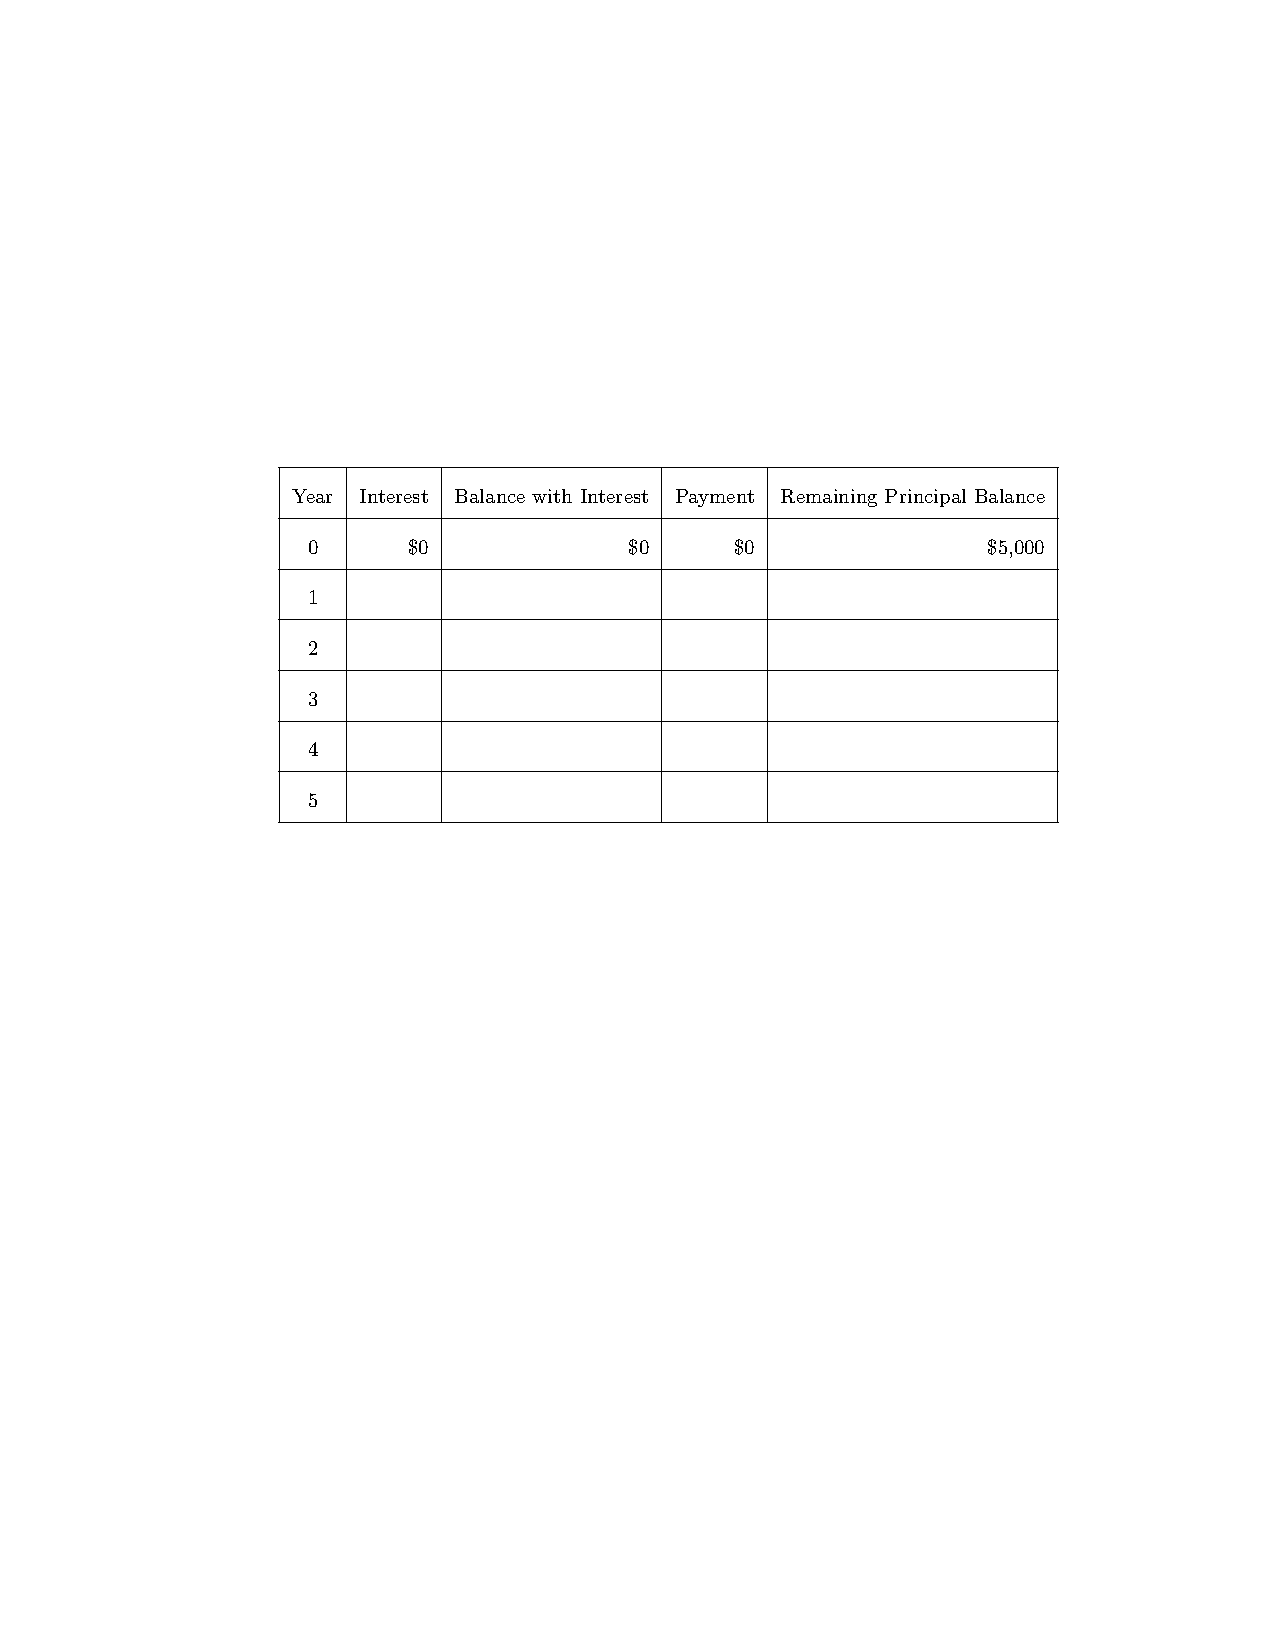
\includegraphics{payingOffDebtTableGraphic.pdf}</span></td>
      </tr>
      <tr>
        <td id="L50" class="blob-num js-line-number" data-line-number="50"></td>
        <td id="LC50" class="blob-code blob-code-inner js-file-line"><span class="pl-c">%% \end{image}</span></td>
      </tr>
      <tr>
        <td id="L51" class="blob-num js-line-number" data-line-number="51"></td>
        <td id="LC51" class="blob-code blob-code-inner js-file-line"><span class="pl-c">%% \begin{freeResponse}</span></td>
      </tr>
      <tr>
        <td id="L52" class="blob-num js-line-number" data-line-number="52"></td>
        <td id="LC52" class="blob-code blob-code-inner js-file-line"><span class="pl-c">%% \end{freeResponse}</span></td>
      </tr>
      <tr>
        <td id="L53" class="blob-num js-line-number" data-line-number="53"></td>
        <td id="LC53" class="blob-code blob-code-inner js-file-line"><span class="pl-c1">\end</span>{question}</td>
      </tr>
      <tr>
        <td id="L54" class="blob-num js-line-number" data-line-number="54"></td>
        <td id="LC54" class="blob-code blob-code-inner js-file-line">
</td>
      </tr>
      <tr>
        <td id="L55" class="blob-num js-line-number" data-line-number="55"></td>
        <td id="LC55" class="blob-code blob-code-inner js-file-line"><span class="pl-c1">\begin</span>{question}</td>
      </tr>
      <tr>
        <td id="L56" class="blob-num js-line-number" data-line-number="56"></td>
        <td id="LC56" class="blob-code blob-code-inner js-file-line">Based on your table, was your guess is too low, too high, or just</td>
      </tr>
      <tr>
        <td id="L57" class="blob-num js-line-number" data-line-number="57"></td>
        <td id="LC57" class="blob-code blob-code-inner js-file-line">right?</td>
      </tr>
      <tr>
        <td id="L58" class="blob-num js-line-number" data-line-number="58"></td>
        <td id="LC58" class="blob-code blob-code-inner js-file-line"><span class="pl-c1">\begin</span>{multipleChoice}</td>
      </tr>
      <tr>
        <td id="L59" class="blob-num js-line-number" data-line-number="59"></td>
        <td id="LC59" class="blob-code blob-code-inner js-file-line">  <span class="pl-c1">\choice</span>{Too low}</td>
      </tr>
      <tr>
        <td id="L60" class="blob-num js-line-number" data-line-number="60"></td>
        <td id="LC60" class="blob-code blob-code-inner js-file-line">  <span class="pl-c1">\choice</span>[correct]{Too high}</td>
      </tr>
      <tr>
        <td id="L61" class="blob-num js-line-number" data-line-number="61"></td>
        <td id="LC61" class="blob-code blob-code-inner js-file-line">  <span class="pl-c1">\choice</span>{Just right}</td>
      </tr>
      <tr>
        <td id="L62" class="blob-num js-line-number" data-line-number="62"></td>
        <td id="LC62" class="blob-code blob-code-inner js-file-line"><span class="pl-c1">\end</span>{multipleChoice}</td>
      </tr>
      <tr>
        <td id="L63" class="blob-num js-line-number" data-line-number="63"></td>
        <td id="LC63" class="blob-code blob-code-inner js-file-line">
</td>
      </tr>
      <tr>
        <td id="L64" class="blob-num js-line-number" data-line-number="64"></td>
        <td id="LC64" class="blob-code blob-code-inner js-file-line"><span class="pl-c1">\end</span>{question}</td>
      </tr>
      <tr>
        <td id="L65" class="blob-num js-line-number" data-line-number="65"></td>
        <td id="LC65" class="blob-code blob-code-inner js-file-line">
</td>
      </tr>
      <tr>
        <td id="L66" class="blob-num js-line-number" data-line-number="66"></td>
        <td id="LC66" class="blob-code blob-code-inner js-file-line"><span class="pl-c1">\begin</span>{question}<span class="pl-c">%[0in]</span></td>
      </tr>
      <tr>
        <td id="L67" class="blob-num js-line-number" data-line-number="67"></td>
        <td id="LC67" class="blob-code blob-code-inner js-file-line">  <span class="pl-c">%Complete the table again for other possible payment amounts until</span></td>
      </tr>
      <tr>
        <td id="L68" class="blob-num js-line-number" data-line-number="68"></td>
        <td id="LC68" class="blob-code blob-code-inner js-file-line">  <span class="pl-c">%you have found the ``best&#39;&#39; annual payment.  %(In Ximera, enter just</span></td>
      </tr>
      <tr>
        <td id="L69" class="blob-num js-line-number" data-line-number="69"></td>
        <td id="LC69" class="blob-code blob-code-inner js-file-line">  <span class="pl-c">%the last row of your table.)</span></td>
      </tr>
      <tr>
        <td id="L70" class="blob-num js-line-number" data-line-number="70"></td>
        <td id="LC70" class="blob-code blob-code-inner js-file-line">
</td>
      </tr>
      <tr>
        <td id="L71" class="blob-num js-line-number" data-line-number="71"></td>
        <td id="LC71" class="blob-code blob-code-inner js-file-line">  Complete the table again for a payment</td>
      </tr>
      <tr>
        <td id="L72" class="blob-num js-line-number" data-line-number="72"></td>
        <td id="LC72" class="blob-code blob-code-inner js-file-line">  of <span class="pl-s"><span class="pl-pds">$</span><span class="pl-cce">\$</span><span class="pl-c1">1219.45</span><span class="pl-pds">$</span></span>.  Round all answers to the nearest cent.</td>
      </tr>
      <tr>
        <td id="L73" class="blob-num js-line-number" data-line-number="73"></td>
        <td id="LC73" class="blob-code blob-code-inner js-file-line">  <span class="pl-cce">\[</span></td>
      </tr>
      <tr>
        <td id="L74" class="blob-num js-line-number" data-line-number="74"></td>
        <td id="LC74" class="blob-code blob-code-inner js-file-line">  <span class="pl-c1">\begin</span>{array}{|c|c|c|c|c|}</td>
      </tr>
      <tr>
        <td id="L75" class="blob-num js-line-number" data-line-number="75"></td>
        <td id="LC75" class="blob-code blob-code-inner js-file-line">    <span class="pl-c1">\hline</span></td>
      </tr>
      <tr>
        <td id="L76" class="blob-num js-line-number" data-line-number="76"></td>
        <td id="LC76" class="blob-code blob-code-inner js-file-line">    <span class="pl-c1">\text</span>{Year} &amp; <span class="pl-c1">\text</span>{Interest}             &amp; <span class="pl-c1">\text</span>{Balance with Interest} &amp; <span class="pl-c1">\text</span>{Payment}    &amp; <span class="pl-c1">\text</span>{Remaining Principal Balance}<span class="pl-c1">\\</span> <span class="pl-c1">\hline</span></td>
      </tr>
      <tr>
        <td id="L77" class="blob-num js-line-number" data-line-number="77"></td>
        <td id="LC77" class="blob-code blob-code-inner js-file-line">    0  &amp; <span class="pl-cce">\$</span> 0               &amp; ---                   &amp; <span class="pl-cce">\$</span> 0        &amp; <span class="pl-cce">\$</span> 5000 <span class="pl-c1">\\</span> <span class="pl-c1">\hline</span></td>
      </tr>
      <tr>
        <td id="L78" class="blob-num js-line-number" data-line-number="78"></td>
        <td id="LC78" class="blob-code blob-code-inner js-file-line">    1  &amp; <span class="pl-cce">\$</span> <span class="pl-c1">\answer</span>{350}    &amp; <span class="pl-cce">\$</span> <span class="pl-c1">\answer</span>{5350}    &amp; <span class="pl-cce">\$</span> 1219.45  &amp; <span class="pl-cce">\$</span> <span class="pl-c1">\answer</span>{4130.55} <span class="pl-c1">\\</span> <span class="pl-c1">\hline</span></td>
      </tr>
      <tr>
        <td id="L79" class="blob-num js-line-number" data-line-number="79"></td>
        <td id="LC79" class="blob-code blob-code-inner js-file-line">    2  &amp; <span class="pl-cce">\$</span> <span class="pl-c1">\answer</span>{289.14} &amp; <span class="pl-cce">\$</span> <span class="pl-c1">\answer</span>{4419.69} &amp; <span class="pl-cce">\$</span> 1219.45  &amp; <span class="pl-cce">\$</span> <span class="pl-c1">\answer</span>{3200.24} <span class="pl-c1">\\</span> <span class="pl-c1">\hline</span></td>
      </tr>
      <tr>
        <td id="L80" class="blob-num js-line-number" data-line-number="80"></td>
        <td id="LC80" class="blob-code blob-code-inner js-file-line">    3  &amp; <span class="pl-cce">\$</span> <span class="pl-c1">\answer</span>{224.02} &amp; <span class="pl-cce">\$</span> <span class="pl-c1">\answer</span>{3424.26} &amp; <span class="pl-cce">\$</span> 1219.45  &amp; <span class="pl-cce">\$</span> <span class="pl-c1">\answer</span>{2204.81} <span class="pl-c1">\\</span> <span class="pl-c1">\hline</span></td>
      </tr>
      <tr>
        <td id="L81" class="blob-num js-line-number" data-line-number="81"></td>
        <td id="LC81" class="blob-code blob-code-inner js-file-line">    4  &amp; <span class="pl-cce">\$</span> <span class="pl-c1">\answer</span>{154.34} &amp; <span class="pl-cce">\$</span> <span class="pl-c1">\answer</span>{2359.15} &amp; <span class="pl-cce">\$</span> 1219.45  &amp; <span class="pl-cce">\$</span> <span class="pl-c1">\answer</span>{1139.70} <span class="pl-c1">\\</span> <span class="pl-c1">\hline</span></td>
      </tr>
      <tr>
        <td id="L82" class="blob-num js-line-number" data-line-number="82"></td>
        <td id="LC82" class="blob-code blob-code-inner js-file-line">    5  &amp; <span class="pl-cce">\$</span> <span class="pl-c1">\answer</span>{79.78}  &amp; <span class="pl-cce">\$</span> <span class="pl-c1">\answer</span>{1219.48} &amp; <span class="pl-cce">\$</span> 1219.45  &amp; <span class="pl-cce">\$</span> <span class="pl-c1">\answer</span>{0.03} <span class="pl-c1">\\</span> <span class="pl-c1">\hline</span></td>
      </tr>
      <tr>
        <td id="L83" class="blob-num js-line-number" data-line-number="83"></td>
        <td id="LC83" class="blob-code blob-code-inner js-file-line">    <span class="pl-c1">\end</span>{array}</td>
      </tr>
      <tr>
        <td id="L84" class="blob-num js-line-number" data-line-number="84"></td>
        <td id="LC84" class="blob-code blob-code-inner js-file-line">  <span class="pl-cce">\]</span></td>
      </tr>
      <tr>
        <td id="L85" class="blob-num js-line-number" data-line-number="85"></td>
        <td id="LC85" class="blob-code blob-code-inner js-file-line">
</td>
      </tr>
      <tr>
        <td id="L86" class="blob-num js-line-number" data-line-number="86"></td>
        <td id="LC86" class="blob-code blob-code-inner js-file-line"><span class="pl-c">%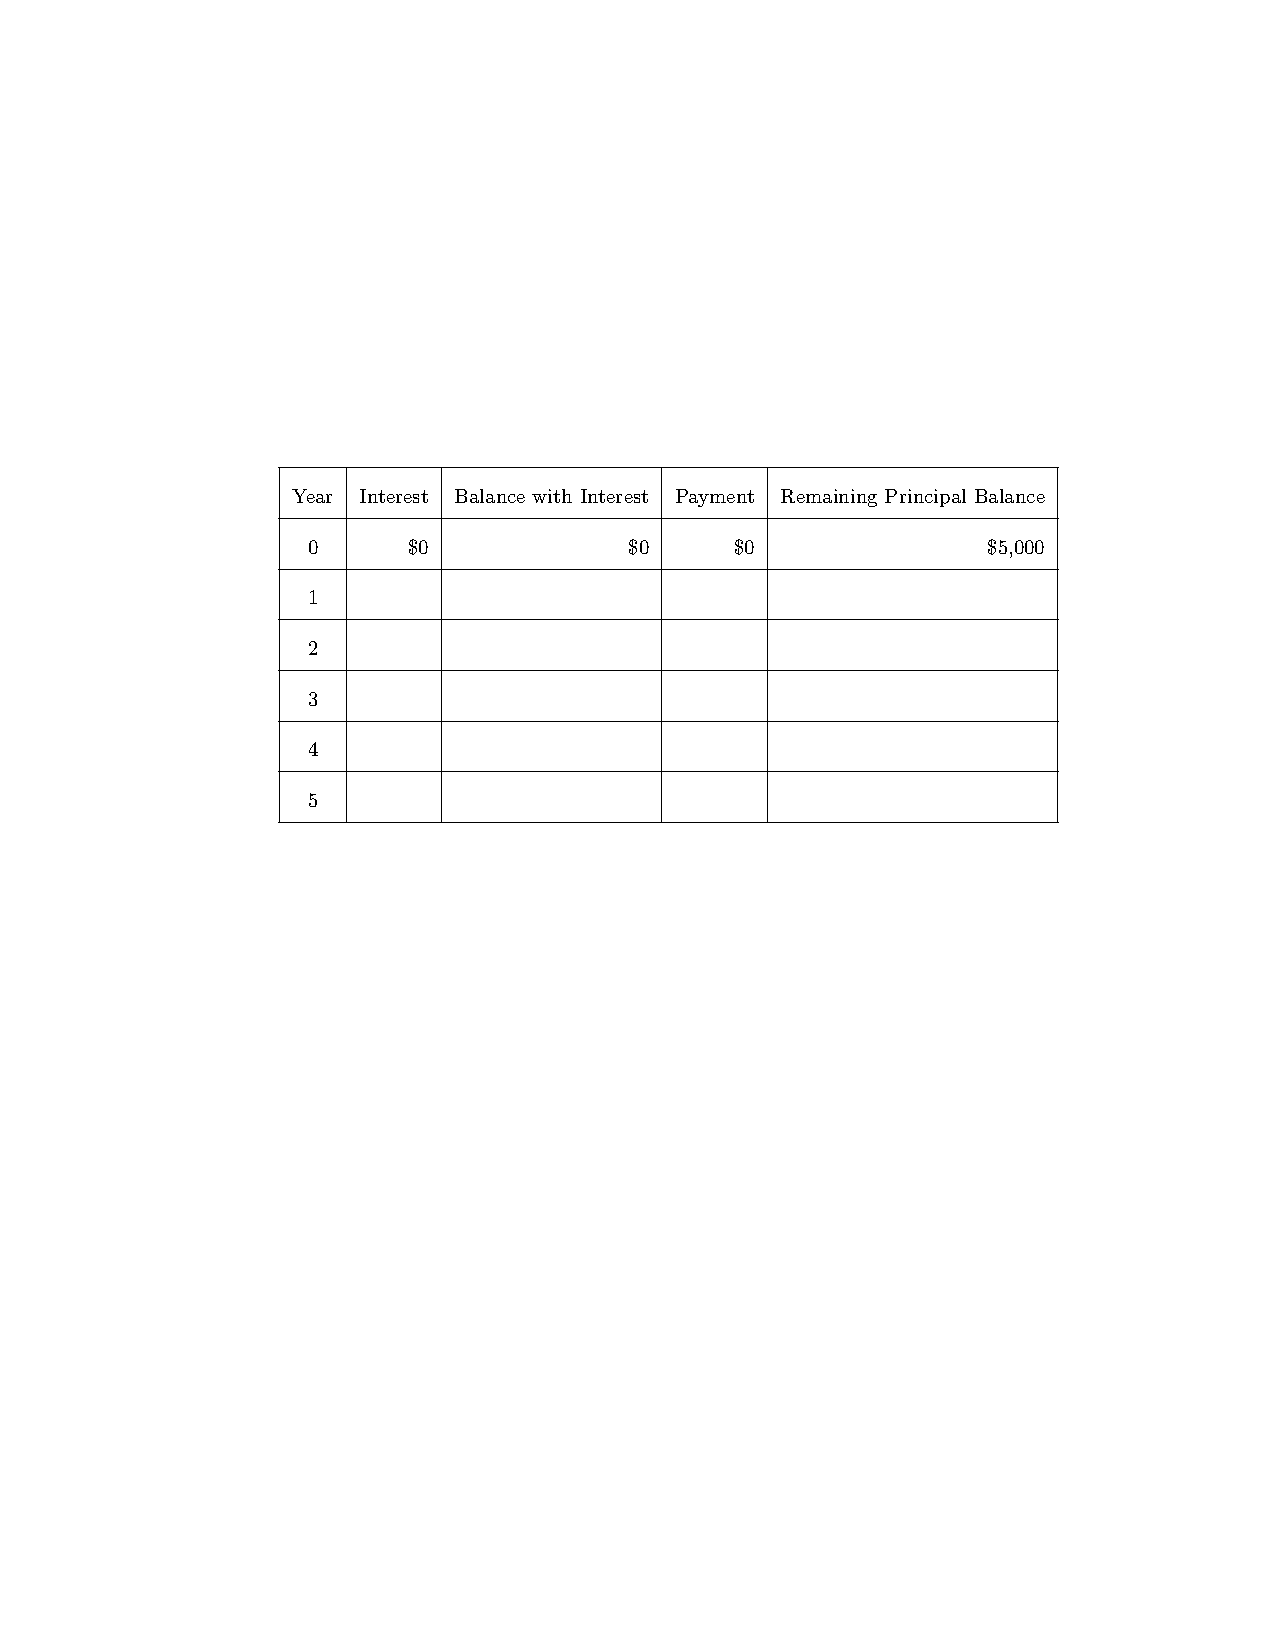
\includegraphics{payingOffDebtTableGraphic.pdf}</span></td>
      </tr>
      <tr>
        <td id="L87" class="blob-num js-line-number" data-line-number="87"></td>
        <td id="LC87" class="blob-code blob-code-inner js-file-line"><span class="pl-c1">\end</span>{question}</td>
      </tr>
      <tr>
        <td id="L88" class="blob-num js-line-number" data-line-number="88"></td>
        <td id="LC88" class="blob-code blob-code-inner js-file-line">
</td>
      </tr>
      <tr>
        <td id="L89" class="blob-num js-line-number" data-line-number="89"></td>
        <td id="LC89" class="blob-code blob-code-inner js-file-line"><span class="pl-c1">\begin</span>{question}</td>
      </tr>
      <tr>
        <td id="L90" class="blob-num js-line-number" data-line-number="90"></td>
        <td id="LC90" class="blob-code blob-code-inner js-file-line">Using your best annual payment, how much interest would you pay in total over the <span class="pl-s"><span class="pl-pds">$</span><span class="pl-c1">5</span><span class="pl-pds">$</span></span> years? </td>
      </tr>
      <tr>
        <td id="L91" class="blob-num js-line-number" data-line-number="91"></td>
        <td id="LC91" class="blob-code blob-code-inner js-file-line"><span class="pl-c1">\begin</span>{prompt}</td>
      </tr>
      <tr>
        <td id="L92" class="blob-num js-line-number" data-line-number="92"></td>
        <td id="LC92" class="blob-code blob-code-inner js-file-line">  You would pay <span class="pl-cce">\$</span> <span class="pl-s"><span class="pl-pds">$</span><span class="pl-c1">\answer</span>{1097.28}<span class="pl-pds">$</span></span>.</td>
      </tr>
      <tr>
        <td id="L93" class="blob-num js-line-number" data-line-number="93"></td>
        <td id="LC93" class="blob-code blob-code-inner js-file-line"><span class="pl-c1">\end</span>{prompt}</td>
      </tr>
      <tr>
        <td id="L94" class="blob-num js-line-number" data-line-number="94"></td>
        <td id="LC94" class="blob-code blob-code-inner js-file-line"><span class="pl-c1">\end</span>{question}</td>
      </tr>
      <tr>
        <td id="L95" class="blob-num js-line-number" data-line-number="95"></td>
        <td id="LC95" class="blob-code blob-code-inner js-file-line">
</td>
      </tr>
      <tr>
        <td id="L96" class="blob-num js-line-number" data-line-number="96"></td>
        <td id="LC96" class="blob-code blob-code-inner js-file-line"><span class="pl-c">%% \begin{question}[.5in]</span></td>
      </tr>
      <tr>
        <td id="L97" class="blob-num js-line-number" data-line-number="97"></td>
        <td id="LC97" class="blob-code blob-code-inner js-file-line"><span class="pl-c">%% Complete the table again, this time with a beginning principal of $P$, an interest rate of $r$,</span></td>
      </tr>
      <tr>
        <td id="L98" class="blob-num js-line-number" data-line-number="98"></td>
        <td id="LC98" class="blob-code blob-code-inner js-file-line"><span class="pl-c">%% and a payment amount of $x$.  Hint: It helps to collect factors of $(1+r)$.</span></td>
      </tr>
      <tr>
        <td id="L99" class="blob-num js-line-number" data-line-number="99"></td>
        <td id="LC99" class="blob-code blob-code-inner js-file-line">
</td>
      </tr>
      <tr>
        <td id="L100" class="blob-num js-line-number" data-line-number="100"></td>
        <td id="LC100" class="blob-code blob-code-inner js-file-line"><span class="pl-c">%% Then write an equation that must be true if $x$ is the correct</span></td>
      </tr>
      <tr>
        <td id="L101" class="blob-num js-line-number" data-line-number="101"></td>
        <td id="LC101" class="blob-code blob-code-inner js-file-line"><span class="pl-c">%% payment amount.   %(In Ximera, enter just the equation.)</span></td>
      </tr>
      <tr>
        <td id="L102" class="blob-num js-line-number" data-line-number="102"></td>
        <td id="LC102" class="blob-code blob-code-inner js-file-line">
</td>
      </tr>
      <tr>
        <td id="L103" class="blob-num js-line-number" data-line-number="103"></td>
        <td id="LC103" class="blob-code blob-code-inner js-file-line"><span class="pl-c">%% 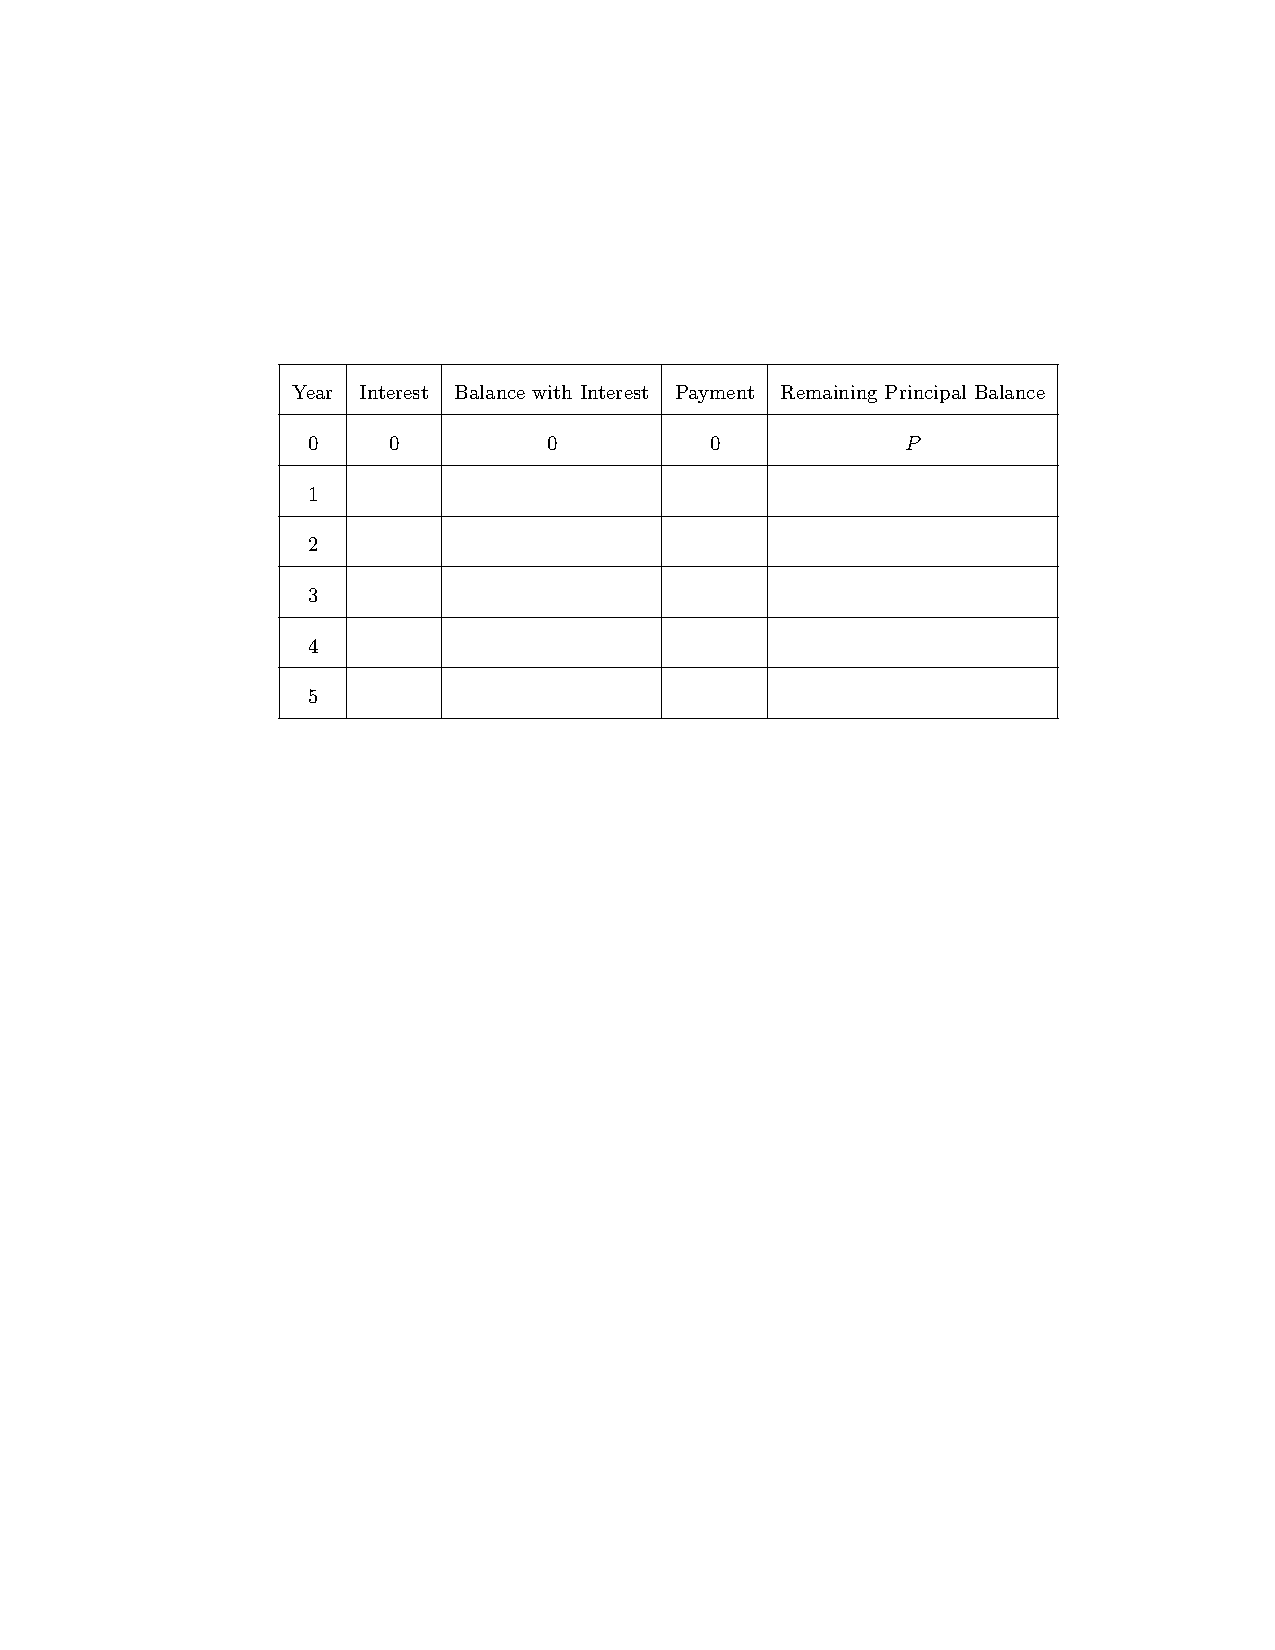
\includegraphics{payingOffDebtTableGraphic2.pdf}</span></td>
      </tr>
      <tr>
        <td id="L104" class="blob-num js-line-number" data-line-number="104"></td>
        <td id="LC104" class="blob-code blob-code-inner js-file-line">
</td>
      </tr>
      <tr>
        <td id="L105" class="blob-num js-line-number" data-line-number="105"></td>
        <td id="LC105" class="blob-code blob-code-inner js-file-line"><span class="pl-c">%% \begin{freeResponse}</span></td>
      </tr>
      <tr>
        <td id="L106" class="blob-num js-line-number" data-line-number="106"></td>
        <td id="LC106" class="blob-code blob-code-inner js-file-line"><span class="pl-c">%% \end{freeResponse}</span></td>
      </tr>
      <tr>
        <td id="L107" class="blob-num js-line-number" data-line-number="107"></td>
        <td id="LC107" class="blob-code blob-code-inner js-file-line"><span class="pl-c">%% \end{question}</span></td>
      </tr>
      <tr>
        <td id="L108" class="blob-num js-line-number" data-line-number="108"></td>
        <td id="LC108" class="blob-code blob-code-inner js-file-line">
</td>
      </tr>
      <tr>
        <td id="L109" class="blob-num js-line-number" data-line-number="109"></td>
        <td id="LC109" class="blob-code blob-code-inner js-file-line"><span class="pl-c">%% \begin{question}</span></td>
      </tr>
      <tr>
        <td id="L110" class="blob-num js-line-number" data-line-number="110"></td>
        <td id="LC110" class="blob-code blob-code-inner js-file-line"><span class="pl-c">%% What is your next question?   </span></td>
      </tr>
      <tr>
        <td id="L111" class="blob-num js-line-number" data-line-number="111"></td>
        <td id="LC111" class="blob-code blob-code-inner js-file-line"><span class="pl-c">%% \begin{freeResponse}</span></td>
      </tr>
      <tr>
        <td id="L112" class="blob-num js-line-number" data-line-number="112"></td>
        <td id="LC112" class="blob-code blob-code-inner js-file-line"><span class="pl-c">%% \end{freeResponse}</span></td>
      </tr>
      <tr>
        <td id="L113" class="blob-num js-line-number" data-line-number="113"></td>
        <td id="LC113" class="blob-code blob-code-inner js-file-line"><span class="pl-c">%% \end{question}</span></td>
      </tr>
      <tr>
        <td id="L114" class="blob-num js-line-number" data-line-number="114"></td>
        <td id="LC114" class="blob-code blob-code-inner js-file-line">
</td>
      </tr>
      <tr>
        <td id="L115" class="blob-num js-line-number" data-line-number="115"></td>
        <td id="LC115" class="blob-code blob-code-inner js-file-line">
</td>
      </tr>
      <tr>
        <td id="L116" class="blob-num js-line-number" data-line-number="116"></td>
        <td id="LC116" class="blob-code blob-code-inner js-file-line"><span class="pl-c">%\begin{question}</span></td>
      </tr>
      <tr>
        <td id="L117" class="blob-num js-line-number" data-line-number="117"></td>
        <td id="LC117" class="blob-code blob-code-inner js-file-line"><span class="pl-c">%Some students notice that the equation above includes a geometric series.  Write the geometric series here.</span></td>
      </tr>
      <tr>
        <td id="L118" class="blob-num js-line-number" data-line-number="118"></td>
        <td id="LC118" class="blob-code blob-code-inner js-file-line"><span class="pl-c">%\begin{freeResponse}</span></td>
      </tr>
      <tr>
        <td id="L119" class="blob-num js-line-number" data-line-number="119"></td>
        <td id="LC119" class="blob-code blob-code-inner js-file-line"><span class="pl-c">%\end{freeResponse}</span></td>
      </tr>
      <tr>
        <td id="L120" class="blob-num js-line-number" data-line-number="120"></td>
        <td id="LC120" class="blob-code blob-code-inner js-file-line"><span class="pl-c">%\end{question}</span></td>
      </tr>
      <tr>
        <td id="L121" class="blob-num js-line-number" data-line-number="121"></td>
        <td id="LC121" class="blob-code blob-code-inner js-file-line"><span class="pl-c">%</span></td>
      </tr>
      <tr>
        <td id="L122" class="blob-num js-line-number" data-line-number="122"></td>
        <td id="LC122" class="blob-code blob-code-inner js-file-line"><span class="pl-c">%\begin{question}</span></td>
      </tr>
      <tr>
        <td id="L123" class="blob-num js-line-number" data-line-number="123"></td>
        <td id="LC123" class="blob-code blob-code-inner js-file-line"><span class="pl-c">%How do you know this is a series?  How do you know this is a geometric series?   </span></td>
      </tr>
      <tr>
        <td id="L124" class="blob-num js-line-number" data-line-number="124"></td>
        <td id="LC124" class="blob-code blob-code-inner js-file-line"><span class="pl-c">%\begin{freeResponse}</span></td>
      </tr>
      <tr>
        <td id="L125" class="blob-num js-line-number" data-line-number="125"></td>
        <td id="LC125" class="blob-code blob-code-inner js-file-line"><span class="pl-c">%\end{freeResponse}</span></td>
      </tr>
      <tr>
        <td id="L126" class="blob-num js-line-number" data-line-number="126"></td>
        <td id="LC126" class="blob-code blob-code-inner js-file-line"><span class="pl-c">%\end{question}</span></td>
      </tr>
      <tr>
        <td id="L127" class="blob-num js-line-number" data-line-number="127"></td>
        <td id="LC127" class="blob-code blob-code-inner js-file-line"><span class="pl-c">%</span></td>
      </tr>
      <tr>
        <td id="L128" class="blob-num js-line-number" data-line-number="128"></td>
        <td id="LC128" class="blob-code blob-code-inner js-file-line"><span class="pl-c">%\begin{question}</span></td>
      </tr>
      <tr>
        <td id="L129" class="blob-num js-line-number" data-line-number="129"></td>
        <td id="LC129" class="blob-code blob-code-inner js-file-line"><span class="pl-c">%Call the geometric series $S$, and note that if you multiply $S$ by $1.07$, the ``common ratio,&#39;&#39; you get another geometric series with many of the same terms.  Use these observations to find the sum of the series.   </span></td>
      </tr>
      <tr>
        <td id="L130" class="blob-num js-line-number" data-line-number="130"></td>
        <td id="LC130" class="blob-code blob-code-inner js-file-line"><span class="pl-c">%\begin{freeResponse}</span></td>
      </tr>
      <tr>
        <td id="L131" class="blob-num js-line-number" data-line-number="131"></td>
        <td id="LC131" class="blob-code blob-code-inner js-file-line"><span class="pl-c">%\end{freeResponse}</span></td>
      </tr>
      <tr>
        <td id="L132" class="blob-num js-line-number" data-line-number="132"></td>
        <td id="LC132" class="blob-code blob-code-inner js-file-line"><span class="pl-c">%\end{question}</span></td>
      </tr>
      <tr>
        <td id="L133" class="blob-num js-line-number" data-line-number="133"></td>
        <td id="LC133" class="blob-code blob-code-inner js-file-line">
</td>
      </tr>
      <tr>
        <td id="L134" class="blob-num js-line-number" data-line-number="134"></td>
        <td id="LC134" class="blob-code blob-code-inner js-file-line">
</td>
      </tr>
      <tr>
        <td id="L135" class="blob-num js-line-number" data-line-number="135"></td>
        <td id="LC135" class="blob-code blob-code-inner js-file-line"><span class="pl-c1">\end</span>{document}</td>
      </tr>
</table>

  </div>

</div>

<button type="button" data-facebox="#jump-to-line" data-facebox-class="linejump" data-hotkey="l" class="hidden">Jump to Line</button>
<div id="jump-to-line" style="display:none">
  <!-- </textarea> --><!-- '"` --><form accept-charset="UTF-8" action="" class="js-jump-to-line-form" method="get"><div style="margin:0;padding:0;display:inline"><input name="utf8" type="hidden" value="&#x2713;" /></div>
    <input class="linejump-input js-jump-to-line-field" type="text" placeholder="Jump to line&hellip;" aria-label="Jump to line" autofocus>
    <button type="submit" class="btn">Go</button>
</form></div>

  </div>
  <div class="modal-backdrop"></div>
</div>


    </div>
  </div>

    </div>

        <div class="container site-footer-container">
  <div class="site-footer" role="contentinfo">
    <ul class="site-footer-links right">
        <li><a href="https://status.github.com/" data-ga-click="Footer, go to status, text:status">Status</a></li>
      <li><a href="https://developer.github.com" data-ga-click="Footer, go to api, text:api">API</a></li>
      <li><a href="https://training.github.com" data-ga-click="Footer, go to training, text:training">Training</a></li>
      <li><a href="https://shop.github.com" data-ga-click="Footer, go to shop, text:shop">Shop</a></li>
        <li><a href="https://github.com/blog" data-ga-click="Footer, go to blog, text:blog">Blog</a></li>
        <li><a href="https://github.com/about" data-ga-click="Footer, go to about, text:about">About</a></li>
          <li><a href="https://github.com/pricing" data-ga-click="Footer, go to pricing, text:pricing">Pricing</a></li>

    </ul>

    <a href="https://github.com" aria-label="Homepage" class="site-footer-mark">
      <svg aria-hidden="true" class="octicon octicon-mark-github" height="24" role="img" title="GitHub " version="1.1" viewBox="0 0 16 16" width="24"><path d="M8 0C3.58 0 0 3.58 0 8c0 3.54 2.29 6.53 5.47 7.59 0.4 0.07 0.55-0.17 0.55-0.38 0-0.19-0.01-0.82-0.01-1.49-2.01 0.37-2.53-0.49-2.69-0.94-0.09-0.23-0.48-0.94-0.82-1.13-0.28-0.15-0.68-0.52-0.01-0.53 0.63-0.01 1.08 0.58 1.23 0.82 0.72 1.21 1.87 0.87 2.33 0.66 0.07-0.52 0.28-0.87 0.51-1.07-1.78-0.2-3.64-0.89-3.64-3.95 0-0.87 0.31-1.59 0.82-2.15-0.08-0.2-0.36-1.02 0.08-2.12 0 0 0.67-0.21 2.2 0.82 0.64-0.18 1.32-0.27 2-0.27 0.68 0 1.36 0.09 2 0.27 1.53-1.04 2.2-0.82 2.2-0.82 0.44 1.1 0.16 1.92 0.08 2.12 0.51 0.56 0.82 1.27 0.82 2.15 0 3.07-1.87 3.75-3.65 3.95 0.29 0.25 0.54 0.73 0.54 1.48 0 1.07-0.01 1.93-0.01 2.2 0 0.21 0.15 0.46 0.55 0.38C13.71 14.53 16 11.53 16 8 16 3.58 12.42 0 8 0z"></path></svg>
</a>
    <ul class="site-footer-links">
      <li>&copy; 2016 <span title="0.05043s from github-fe116-cp1-prd.iad.github.net">GitHub</span>, Inc.</li>
        <li><a href="https://github.com/site/terms" data-ga-click="Footer, go to terms, text:terms">Terms</a></li>
        <li><a href="https://github.com/site/privacy" data-ga-click="Footer, go to privacy, text:privacy">Privacy</a></li>
        <li><a href="https://github.com/security" data-ga-click="Footer, go to security, text:security">Security</a></li>
        <li><a href="https://github.com/contact" data-ga-click="Footer, go to contact, text:contact">Contact</a></li>
        <li><a href="https://help.github.com" data-ga-click="Footer, go to help, text:help">Help</a></li>
    </ul>
  </div>
</div>



    
    
    

    <div id="ajax-error-message" class="ajax-error-message flash flash-error">
      <svg aria-hidden="true" class="octicon octicon-alert" height="16" role="img" version="1.1" viewBox="0 0 16 16" width="16"><path d="M15.72 12.5l-6.85-11.98C8.69 0.21 8.36 0.02 8 0.02s-0.69 0.19-0.87 0.5l-6.85 11.98c-0.18 0.31-0.18 0.69 0 1C0.47 13.81 0.8 14 1.15 14h13.7c0.36 0 0.69-0.19 0.86-0.5S15.89 12.81 15.72 12.5zM9 12H7V10h2V12zM9 9H7V5h2V9z"></path></svg>
      <button type="button" class="flash-close js-flash-close js-ajax-error-dismiss" aria-label="Dismiss error">
        <svg aria-hidden="true" class="octicon octicon-x" height="16" role="img" version="1.1" viewBox="0 0 12 16" width="12"><path d="M7.48 8l3.75 3.75-1.48 1.48-3.75-3.75-3.75 3.75-1.48-1.48 3.75-3.75L0.77 4.25l1.48-1.48 3.75 3.75 3.75-3.75 1.48 1.48-3.75 3.75z"></path></svg>
      </button>
      Something went wrong with that request. Please try again.
    </div>


      
      <script crossorigin="anonymous" integrity="sha256-vr53zzxq1gM+ffhaV5UrFY0dD62+NZCvGalgsAQTu+w=" src="https://assets-cdn.github.com/assets/frameworks-bebe77cf3c6ad6033e7df85a57952b158d1d0fadbe3590af19a960b00413bbec.js"></script>
      <script async="async" crossorigin="anonymous" integrity="sha256-kFGJaRpgKPiM2AIQhRqN3lA1iG/pSn3NZMhTo0LRZfw=" src="https://assets-cdn.github.com/assets/github-905189691a6028f88cd80210851a8dde5035886fe94a7dcd64c853a342d165fc.js"></script>
      
      
      
    <div class="js-stale-session-flash stale-session-flash flash flash-warn flash-banner hidden">
      <svg aria-hidden="true" class="octicon octicon-alert" height="16" role="img" version="1.1" viewBox="0 0 16 16" width="16"><path d="M15.72 12.5l-6.85-11.98C8.69 0.21 8.36 0.02 8 0.02s-0.69 0.19-0.87 0.5l-6.85 11.98c-0.18 0.31-0.18 0.69 0 1C0.47 13.81 0.8 14 1.15 14h13.7c0.36 0 0.69-0.19 0.86-0.5S15.89 12.81 15.72 12.5zM9 12H7V10h2V12zM9 9H7V5h2V9z"></path></svg>
      <span class="signed-in-tab-flash">You signed in with another tab or window. <a href="">Reload</a> to refresh your session.</span>
      <span class="signed-out-tab-flash">You signed out in another tab or window. <a href="">Reload</a> to refresh your session.</span>
    </div>
    <div class="facebox" id="facebox" style="display:none;">
  <div class="facebox-popup">
    <div class="facebox-content" role="dialog" aria-labelledby="facebox-header" aria-describedby="facebox-description">
    </div>
    <button type="button" class="facebox-close js-facebox-close" aria-label="Close modal">
      <svg aria-hidden="true" class="octicon octicon-x" height="16" role="img" version="1.1" viewBox="0 0 12 16" width="12"><path d="M7.48 8l3.75 3.75-1.48 1.48-3.75-3.75-3.75 3.75-1.48-1.48 3.75-3.75L0.77 4.25l1.48-1.48 3.75 3.75 3.75-3.75 1.48 1.48-3.75 3.75z"></path></svg>
    </button>
  </div>
</div>

  </body>
</html>

